\thispagestyle{empty}
\subsection*{\huge Invocador}
\vspace{0.3cm}
"No me gusta tu plan. Apesta." \\
\indent -- Yuna 
\vspace{0.3cm} \\
Los Invocadores son poderosos hechiceros que pueden invocar bestias mágicas para que los asistan en combate. Crean un fuerte vínculo con su invocación, que permite al Invocador controlar sus increíbles poderes a voluntad. Aunque los Invocadores se centran en usar magia defensiva, sus invocaciones pueden causar más estragos que cualquier ser humano.
\vfill
\battrt{ \textbf{Nivel 1:} & PV~+16 & PM~+19 & AGI~+2 & MAG~+1 \\ 
 \textbf{Nivel 2:} & PV~+5 & PM~+10 & RES~+1 & FUE~+1 \\ 
 \textbf{Nivel 3:} & PV~+10 & PM~+10 & MAG~+1 &         
}{Bastón}{Túnica}
\vfill
\atypet{Devoto} { \textbf{Nivel 4:} & PV~+5 & PM~+10 & RES~+1 & DEF~+1 \\  
 \textbf{Nivel 5:} & PV~+10 & PM~+10 & MAG~+1 &        \\  
 \textbf{Nivel 6:} & PV~+5 & PM~+10 & MAG~+1 & RES~+1 \\  
 \textbf{Nivel 7:} & PV~+5 & PM~+10 & RES~+2 &        \\  
 \textbf{Nivel 8:} & PV~+10 & PM~+10 & DEF~+1 &		  \\  
 \textbf{Nivel 9:} & PV~+5 & PM~+10 & MAG~+1 & RES~+1 \\  
 \textbf{Nivel 10:}& PV~+10 & PM~+10 & MAG~+1 &        \\  
} {Unión de Almas} { En tu turno, la invocación que esté activa puede lanzar un hechizo utilizando tus PM además de los suyos y el tiempo de lanzamiento del hechizo se reduce en 1 turno. Debes omitir tu propio turno para utilizar este efecto. } {Sacrificio} { Siempre que tu invocación activa reciba algún daño, puedes elegir reducir tus propios PV en su lugar. }
\vfill
\atypet{Evocador} { \textbf{Nivel 4:} & PV~+10 & PM~+5 & MAG~+1 & DEF~+1 \\  
 \textbf{Nivel 5:} & PV~+10 & PM~+10 & RES~+1 &		  \\  
 \textbf{Nivel 6:} & PV~+5 & PM~+10 & MAG~+1 & RES~+1 \\  
 \textbf{Nivel 7:} & PV~+10 & PM~+5 & DEF~+1 & RES~+1 \\  
 \textbf{Nivel 8:} & PV~+5 & PM~+10 & MAG~+2 &	      \\  
 \textbf{Nivel 9:} & PV~+5 & PM~+10 & RES~+1 & MAG~+1 \\  
 \textbf{Nivel 10:}& PV~+10 & PM~+10 & RES~+1 &		  \\  
} {Canalizar} {En tu turno, puedes elegir lanzar un hechizo de tu invocación activa. El tiempo de lanzamiento del hechizo se reduce en 1 turno. La invocación debe omitir su turno para poder utilizar este efecto. } {Lazo Vital} { Siempre que recibas algún daño, puedes elegir reducir los PV de tu invocación activa en vez de los tuyos. }
\pagebreak \\
\noindent {\Large\color{accent}\bf \uline{Habilidades\phantom{y}\hfill}}\\\\
\spellt{Invocar}{8}{3t}{Único}{Tú} { Invocas a una criatura que actúa junto a ti en tu turno siguiendo tus instrucciones. La invocación desaparece cuando tú o la invocación pasen a estar \hyperlink{status}{KO}, pero también puedes cancelarla cuando desees. Una vez que la invocación sea cancelada o derrotada, no podrás volver a invocar a la misma criatura en ese mismo día. Todas las criaturas que puedes invocar en tus diferentes niveles de personaje se muestran en la página siguiente. }{}{1} \spellt{Plegaria}{5}{1t}{1u}{Tú}{ Todos los que se encuentren en el área de efecto recuperan 1d de PV. }{}{2} \spellt{Imagen}{10}{1t}{1u}{3u}{ El objetivo obtiene \hyperlink{status}{Reflejos} por 3 turnos. }{\blink}{4} \spellt{Rana}{16}{1t}{Único}{3u}{ El objetivo debe hacer una tirada con DC 8. Si falla, queda convertido en una rana por 3 turnos o hasta que reciba daño. Mientras esté convertido en rana, el objetivo no puede hablar ni realizar ninguna acción y solo puede moverse 1u por turno. }{}{6} \spellt{Disipar}{20}{1t}{Único}{3u}{ Eliminas todas las \hyperlink{type}{Resistencias} e \hyperlink{status}{Inmunidades} del objetivo por 3 turnos. Además, se eliminan todos los \hyperlink{status}{Estados Alterados} beneficiosos que estén activos en el objetivo cuando este hechizo tenga efecto. }{}{8} \spellt{Invocación Gemela}{28}{5t}{Único}{Tú}{ Invocas a dos criaturas que actúan junto a ti en tu turno siguiendo tus instrucciones. Las invocaciones desaparecen cuando tú o las invocaciones pasen a estar \hyperlink{status}{KO}, pero también puedes cancelarla cuando desees. Una vez que la invocación sea cancelada o derrotada, no podrás volver a invocar a la misma criatura en ese mismo día. Todas las criaturas que puedes invocar en tus diferentes niveles de personaje se muestran en la página siguiente. }{}{10}
\vspace{5cm}
\pagebreak
\onecolumn
\noindent{\LARGE\color{accent}\bf \uline{Invocaciones\hfill} \\} \\
\thispagestyle{empty}

\begin{multicols}{2}
\friendly{Carbuncle}{1}{
\includegraphics[width=0.18\textwidth]{./art/monsters/carbuncle.png}}
{ PV: & \hfill 20 & PM: & \hfill 36\\
 FUE: & \hfill 1 & DEF: & \hfill 0 \\
 MAG: & \hfill 2 & RES: & \hfill 2 \\
 AGI: & \hfill 3 & Tamaño: & \hfill P\\
} { \textbf{Tacleo}: 1d de daño\phantom{y} \mspell{Espejo}{12}{1t}{Único}{3u}{El objetivo recibe un escudo mágico que hace rebotar el próximo hechizo que le lancen y se lo devuelve al lanzador.}{} }
\vspace{0.5cm} 
\friendly{Ifrit}{3}{
\includegraphics[width=0.23\textwidth]{./art/monsters/ifrit.png}}
{ PV: & \hfill 50 & PM: & \hfill 36\\
 FUE: & \hfill 2 & DEF: & \hfill 3 \\
 MAG: & \hfill 1 & RES: & \hfill 0 \\
 AGI: & \hfill 3 & Tamaño: & \hfill M\\
} { \textbf{Garra}: 2d de daño \\
 \textbf{Resistencia}:\fire \hfill \textbf{Debilidad:}\ice \mspell{Piro}{4}{1t}{Único}{3u}{Infliges 2d de daño de \hyperlink{fire}{Fuego} al objetivo.}{\fire} \mtech{Fuego Infernal}{12}{1t}{2u}{Tú}{Infliges 4d de daño de \hyperlink{type}{Fuego} a todos los que se encuentren en el área de efecto excepto a ti.}{\fire} }
\vspace{0.5cm} 
\friendly{Shiva}{5}{
\includegraphics[width=0.18\textwidth]{./art/monsters/shiva.png}}
{ PV: & \hfill 60 & PM: & \hfill 80\\
 FUE: & \hfill 1 & DEF: & \hfill 1 \\
 MAG: & \hfill 5 & RES: & \hfill 4 \\
 AGI: & \hfill 3 & Tamaño: & \hfill M\\
} { \textbf{Témpano}: 2d de daño, 3u de alcance \\
 \textbf{Resistencia}:\ice \hspace*{\fill} \textbf{Debilidad:}\fire \mspell{AntiEscudo}{5}{1t}{Único}{3u}{El objetivo sufre \hyperlink{status}{disDEF} por 3 turnos.}{\dedef} \mspell{AntiCoraza}{5}{1t}{Único}{3u}{El objetivo sufre \hyperlink{status}{disRES} por 3 turnos.}{\deres} \mtech{Muro de Hielo}{10}{1t}{3u (línea)}{3u}{ Creas un muro de hielo de 3u de alto y ancho que bloquea el paso por 5 turnos. El muro se rompe después de 5 turnos o tras sufrir un total de 30 puntos de daño. }{} \mspell{Polvo de Diamante}{20}{1t}{3u (frente)}{Tú}{ Todos los enemigos en el área de efecto reciben 6d de daño de \hyperlink{type}{Hielo} y quedan \hyperlink{status}{Inmóviles} por 1 turno. }{\ice\immobile} } \friendly{Fénix}{7}{
\includegraphics[width=0.2\textwidth]{./art/monsters/phoenix.png}}
{ PV: & \hfill 70 & PM: & \hfill 90\\
 FUE: & \hfill 0 & DEF: & \hfill 2 \\
 MAG: & \hfill 6 & RES: & \hfill 8 \\
 AGI: & \hfill 2 & Tamaño: & \hfill M\\
} { \textbf{Picotazo}: 1d de daño \\ 
 \textbf{Inmune}: \hyperlink{status}{Todos los Estados Alterados} \hfill \newline\textbf{Resistencia:}\fire\holy \mspell{Escudo}{5}{1t}{Único}{3u}{El objetivo recibe \hyperlink{status}{aumDEF} por 3 turnos.}{\enndef} \mspell{Coraza}{5}{1t}{Único}{3u}{El objetivo recibe \hyperlink{status}{aumRES} por 3 turnos.}{\enres} \mspell{Cura++}{18}{1t}{1u}{3u}{Todos los que se encuentren en el área de efecto recuperan 6d PV.}{} \mspell{Lázaro+}{28}{3t}{Único}{3u}{Elimina el estado \hyperlink{status}{KO} del objetivo y recupera completamente sus PV.}{\ko} }
\vspace{0.5cm} 
\friendly{Bahamut}{9}{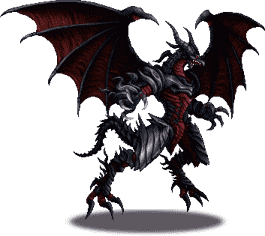
\includegraphics[width=0.23\textwidth]{./art/monsters/bahamut.png}}
{ PV: & \hfill 100 & PM: & \hfill 140\\
 FUE: & \hfill 8 & DEF: & \hfill 6 \\
 MAG: & \hfill 7 & RES: & \hfill 4 \\
 AGI: & \hfill 4 & Tamaño: & \hfill G\\
} { \textbf{Garra}: 3d de daño, 2u de alcance \\
 \textbf{Inmune}: \hyperlink{status}{Todos los Estados Alterados} \hfill \textbf{Resistencia:}\dark \mtech{Aliento Destructor}{20}{1t}{3u (frente)}{3u}{ Todos los que se encuentren en el área de efecto deben hacer una tirada con DC 8. Si fallan, reciben 4d de daño. Además, quedan \hyperlink{status}{Envenenados} y \hyperlink{status}{Ciegos} por 3 turnos. }{\poison \blind} \mspell{Desterrar}{30}{1t}{Único}{3u}{ El objetivo hace una tirada con DC 8. Si falla, es desterrado a otra dimensión, desapareciendo del campo de batalla por 3 turnos. }{} \mspell{Megafulgor}{40}{3t}{Único}{8u}{ Infliges 10d+20 de daño de \hyperlink{type}{Fuego} al objetivo. }{\fire} \mreaction{Ataque Final}{Si tus PV están a punto de llegar a 0, puedes usar una de tus habilidades sin costo ni tiempo de preparación antes de quedar \hyperlink{status}{KO}.} }
\end{multicols}
\twocolumn